% !Mode:: "TeX:UTF-8"
\chapter{Backend: Part I}
\label{cpt:backend1}
\begin{mdframed}  
	\textbf{Goal of Study}
	\begin{enumerate}[labelindent=0em,leftmargin=1.5em]
		\item Learn how to formulate the backend problem into a filter or least square optimization problem.
		\item Learn how to use the sparse structure in bundle adjustment problem. 
		\item Solve a BA problem with g2o and Ceres.
	\end{enumerate}
\end{mdframed}

From this lecture, we turn to another important module: back-end optimization.
We see that the front-end visual odometry can give a short-term trajectory and map. Still, due to the inevitable accumulation of errors, this map is inaccurate for a long time. Therefore, based on visual odometry, we also hope to construct a larger-scale optimization problem to consider the optimal trajectory and map over a long time. However, considering the balance of accuracy and performance, there are many different approaches in practice.

\newpage
\includepdf{resources/other/ch10.pdf}

\newpage
\section{Introduction}
\subsection{State Estimation from Probabilistic Perspective}
As mentioned in the second lecture, the visual odometry only has a short memory, but we hope that the system can maintain the entire motion trajectory in an optimal state for a long time. We may use the latest knowledge to update an old state. At that time, it seems that future information tells you, ``where you should be now.'' Therefore, in the back-end optimization, we usually consider the problem of state estimation for a longer period of time (or all-time), and not only use the past information to update our current state but also use future information to update ourselves. Such a method might be called ``Batch.'' Otherwise, if the current state is only determined by the past, or even only by the previous moment, it might also be called ``Incremental.''

We already know that the SLAM process can be described by the motion and observation equations. Suppose in the time from $t=0$ to $t=N$, we have the poses from $\mathbf{x}_0$ to $\mathbf{x}_N$ and observation $\mathbf{y}_1, \cdots, \mathbf{y}_M$. According to the equations in chapter 2, we write them as: 
\begin{equation}
	\left\{ \begin{array}{l}
		{\mathbf{x}_k} = f\left( {{\mathbf{x}_{k - 1}},{\mathbf{u}_k}} \right) + \mathbf{w}_k \\
		{\mathbf{z}_{k,j}} = h\left( {{ \mathbf{y}_j},{ \mathbf{x}_k}}  \right)+ \mathbf{v}_{k,j}
	\end{array} \right. \quad k=1, \ldots, N, \  j=1, \ldots, M.
\end{equation}

Note that in the SLAM problem we have the following characteristics:
\begin{enumerate}
	\item In the observation equation, only when $\mathbf{x}_k$ sees $\mathbf{y}_j$, we will have a real observation equation. In fact, we can usually see only a small part of the landmarks in one location. Moreover, due to a large number of visual SLAM feature points, the number of observation equations in practice will be much larger than that of motion equations.
	\item We may not have a device to measure the motion, so there may not be a motion equation. In this case, there are several ways to deal with it:
	\begin{itemize}
		\item Assume that there is really no motion equation.
		\item Assume that the camera does not move.
		\item Assume that the camera is moving at a constant speed.
	\end{itemize}
	These several methods are all feasible. In the absence of motion equations, the entire optimization problem consists of only observation equations. This is very similar to the SfM (Structure from Motion) problem, which is equivalent to restoring the motion and structure through a set of images. The difference with SfM is that the images in SLAM have a chronological order, while SfM allows the use of completely unrelated images.
\end{enumerate} 

We know that every measurement is affected by noise, so the poses $\mathbf{x}$ and landmarks $\mathbf{y}$ here are regarded as \textbf{random variables that obey a certain probability distribution} instead of a single number. Therefore, the question becomes: when I have some motion data $\mathbf{u}$ and observation data $\mathbf{z}$, how to determine the state $\mathbf{x}$ and landmarks $\mathbf{y}$'s distribution? Furthermore, if new data is obtained, how to update our estimation? In more common and reasonable cases, we assume that the state quantity and noise terms obey Gaussian distribution-which means that only their mean and covariance matrix need to be stored in the program. The mean can be regarded as an estimate of the state variable's optimal value, and the covariance matrix measures its uncertainty. Then, the question becomes: when there are some motion and observation data, how do we estimate the Gaussian distribution of the states?

We still put ourselves in the role of a robot. When there is only the equation of motion, it is equivalent to walking blindfolded in an unknown place. Although we know how far we have taken for each step, we will become more and more uncertain about where we are as time grows. This reflects that when the input data is affected by noise, the error is gradually accumulated, and our estimate of the position variance will become larger and larger. However, when we open our eyes, we will become more and more confident because we can continuously observe the external scene, making the uncertainty of position estimation smaller. If we use an ellipse to intuitively express the covariance matrix, then this process is a bit like walking in a mobile phone map software. Taking \autoref{fig:uncertainty}~ as an example, readers can imagine that when there is no observation data, the circle will become larger and larger with the movement; and if there are correct observations, the circle will shrink to a certain size and keep stable.

\begin{figure}[!ht]
	\centering
	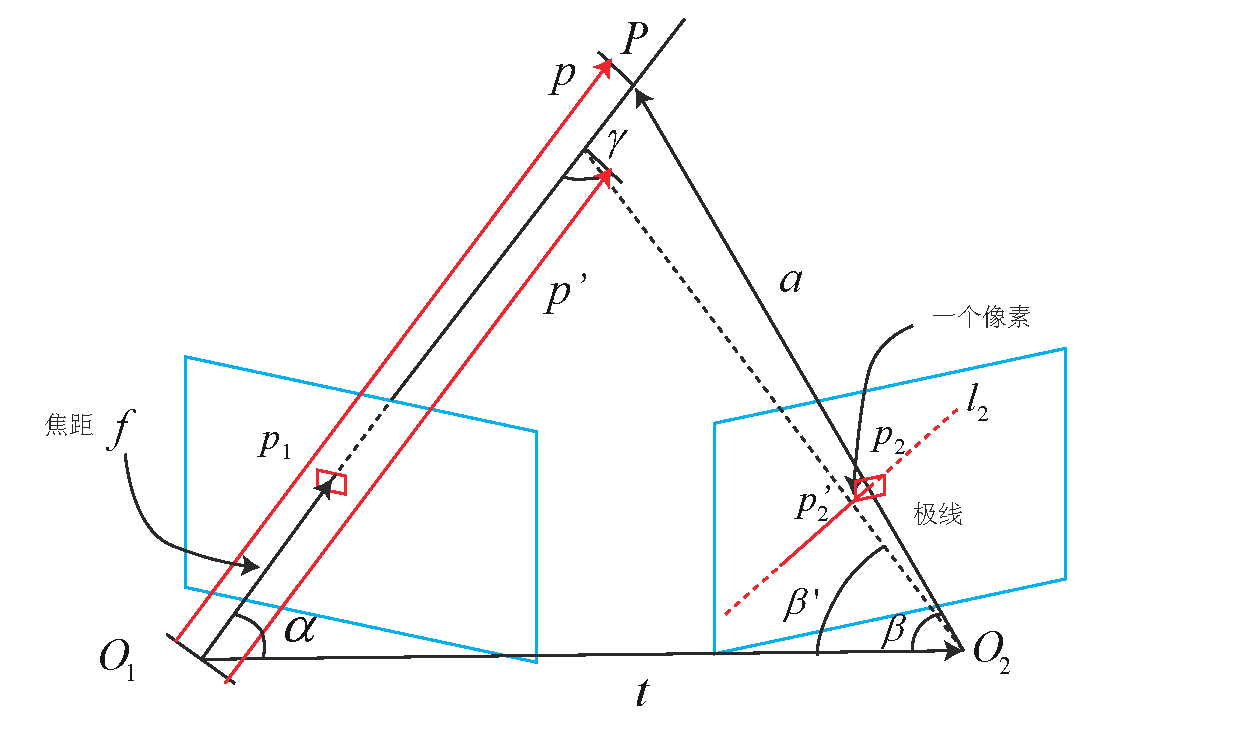
\includegraphics[width=0.66\textwidth]{backend1/uncertainty.pdf}
	\caption{An intuitive description of uncertainty. Left: When there is only the motion equation, the pose at the next moment adds noise to the previous moment, so the uncertainty is getting bigger and bigger. Right: When there are road signs, the uncertainty will be significantly reduced. Please note that this is only an intuitive diagram, not actual data.}
	\label{fig:uncertainty}
\end{figure}

The above statements explain the problem of state estimation in a metaphorical form. Below we will look at it in a quantitative way. In Lecture \ref{cpt:6}, we introduced the maximum likelihood estimation where we say that the problem of \textbf{batch state estimation} can be transformed into a \textbf{maximum likelihood estimation problem and solved by the least square method}. In this section, we will explore how to apply this conclusion to progressive problems and get some classic conclusions. At the same time, we will investigate the special structure of the least square method in visual SLAM.

First of all, since the poses and landmarks are all optimize variables, we change the notation a bit and let $\mathbf{x}_k$ be all the unknowns at the moment of $k$. It contains the current camera pose and $m$ landmarks. With a little abuse of the notation, we rewrite the equations into:
\begin{equation}
	\mathbf{x}_k  \buildrel \Delta \over =  \{ \mathbf{x}_k, \mathbf{y}_1, \ldots, \mathbf{y}_m \}.
\end{equation}

At the same time, all observations at time $k$ are denoted as $\mathbf{z}_k$. Therefore, we can write the motion and observation equations more concisely. There will be no $\mathbf{y}$ here, but we should remember that the previous $\mathbf{y}$ is already included in the $\mathbf{x}$:
\begin{equation}
	\left\{ \begin{array}{l}
		{\mathbf{x}_k} = f\left( {{\mathbf{x}_{k - 1}},{\mathbf{u}_k}} \right) + \mathbf{w}_k \\
		{\mathbf{z}_{k}} = h\left( \mathbf{x}_k  \right)+ \mathbf{v}_{k}
	\end{array} \right. \quad k=1, \ldots, N .
\end{equation}

Now consider the situation at time $k$. We hope to use the data from $0$ to $k$ to estimate the current state distribution:
\begin{equation}
	P(\mathbf{x}_k | \mathbf{x}_0, \mathbf{u}_{1:k}, \mathbf{z}_{1:k}).
\end{equation}

The subscript $0:k$ represents all the data from time $0$ to time $k$. Please note that $\mathbf{z}_k$ represents all the observation data at time $k$. It may be more than one, but we use a single notation here. At the same time, also note that $\mathbf{x}_k$ is related to the previous states like $\mathbf{x}_{k-1}, \mathbf{x}_{k-2}$, but this formula does not explicitly write them out.

Let's see how to do the state estimation. According to Bayes' rule, swap the positions of $\mathbf{z}_k$ and $\mathbf{x}_k$, we have:
\begin{equation}
	\label{eq:10-5}
	P\left( {{\mathbf{x}_k}|{\mathbf{x}_0},{\mathbf{u}_{1:k}},{\mathbf{z}_{1:k}}} \right) \propto \underbrace{P\left( {{\mathbf{z}_k}|{\mathbf{x}_k}} \right)}_{\text{likelihood}} \underbrace{P\left( {{\mathbf{x}_k}|{\mathbf{x}_0},{\mathbf{u}_{1:k}},{\mathbf{z}_{1:k - 1}}} \right)}_{\text{prior}}.
\end{equation}

You may think this is familiar with what we have discussed in the previous sections. Here the first term is called \textbf{likelihood}, and the second term is called \textbf{prior}. The observation equation gives the likelihood. For the prior part, we should know that the current state $\mathbf{x}_k$ is estimated based on all past states. Let's first consider the effect of $\mathbf{x}_{k-1}$. it is expanded according to the conditional probability of $\mathbf{x}_{k-1}$ moment:
\begin{equation}
	\label{eq:bayes-estimator}
	\small
	P\left( {{\mathbf{x}_k}|{\mathbf{x}_0},{\mathbf{u}_{1:k}},{\mathbf{z}_{1:k - 1}}} \right) = \int {P\left( {{\mathbf{x}_k}|{\mathbf{x}_{k - 1}},{\mathbf{x}_0},{\mathbf{u}_{1:k}},{\mathbf{z}_{1:k - 1}}} \right)P\left( {{\mathbf{x}_{k - 1}}|{\mathbf{x}_0},{\mathbf{u}_{1:k}},{\mathbf{z}_{1:k - 1}}} \right) \mathrm{d}\mathbf{x}_{k-1} }.
\end{equation}

There are generally some methodology differences for the next steps: (i) We assume the \textbf{Markov property}. The simple first-order Markov property holds that the state at time $k$ is only related to the state at time $k-1$ and is not related to the earlier states. If such an assumption is made, we will get a filter method represented by \textbf{Extended Kalman Filter} (EKF). In the filtering method, we estimate from the state at a specific moment and derive it to the next moment. (ii) Another technique is to keep the relationship between the state at $k$ and \textbf{all} the previous states (and also, the future states). At this time, we will obtain an optimization framework with \textbf{nonlinear optimization} as the main body. The basic knowledge of nonlinear optimization has been introduced in the previous sections. At present, the mainstream of visual SLAM is to use the nonlinear optimization method. However, in order to make this book more comprehensive, let's first introduce the principles of the Kalman filter and EKF.

\subsection{Linear System and the Kalman Filter}
Let's look at the filter model first. When the Markov property is assumed, what changes will happen from a mathematical perspective? The current state is only related to the previous moment. The first part on the right side of the formula \eqref{eq:bayes-estimator} can be further simplified as:
\begin{equation}
	P\left( {{\mathbf{x}_k}|{\mathbf{x}_{k - 1}},{\mathbf{x}_0},{\mathbf{u}_{1:k}},{\mathbf{z}_{1:k - 1}}} \right) = P\left( {{\mathbf{x}_k}|{\mathbf{x}_{k - 1}},{\mathbf{u}_k}} \right),
\end{equation}
where we omit the states earlier than $k-1$ since they are not related to the $k$-th state. 

The second part can be simplified as: 
\begin{equation}
	P\left( {{\mathbf{x}_{k - 1}}|{\mathbf{x}_0},{\mathbf{u}_{1:k}},{\mathbf{z}_{1:k - 1}}} \right) = P\left( {{\mathbf{x}_{k - 1}}|{\mathbf{x}_0},{\mathbf{u}_{1:k - 1}},{\mathbf{z}_{1:k - 1}}} \right),
\end{equation}
where we drop the $\mathbf{u}_k$ since it has nothing to do with $\mathbf{x}_{k-1}$. 

It can be seen that this item is actually the state distribution at time $k-1$. Therefore, this series of equations shows that what we are actually doing is ``how to derive the state distribution from time $k-1$ to time $k$''. In other words, we only need to maintain the current state estimation and update it incrementally. Furthermore, if it is assumed that the state quantity obeys a Gaussian distribution, we only need to consider the state variable's mean and covariance. You can imagine that the robot's localization module has been outputting two information: the estimated pose (mean) and the uncertainty (covariance), which is exactly the common case in many practical localization libraries.

We start from the simplest linear Gaussian system, and finally, we will reach the famous Kalman filter. A linear Gaussian system is such a system where the motion and observation equations are all linear so that we can write them in a matrix form:
\begin{equation}
	\left\{ \begin{array}{l}
		{\mathbf{x}_k} = \mathbf{A}_k {{\mathbf{x}_{k - 1}}+{\mathbf{u}_k}} + \mathbf{w}_k \\
		{\mathbf{z}_{k}} = \mathbf{C}_k  { \mathbf{x}_k} + \mathbf{v}_{k} \end{array} \right. \quad k=1, \ldots, N ,
\end{equation}
and we assume the states and noises are all Gaussian, so that: 
\begin{equation}
	\mathbf{w}_k \sim N(\mathbf{0}, \mathbf{R}). \quad \mathbf{v}_k \sim N( \mathbf{0}, \mathbf{Q}),
\end{equation}
where we omit the subscripts of $\mathbf{R}$ and $\mathbf{Q}$ for brevity. Now, using the Markov property, suppose we know the posterior state estimation at time $k-1$ $\mathbf{\hat{x}}_{k-1} $ and its covariance $\mathbf{\hat{P}}_{k-1}$, now we want to determine the posterior distribution of $\mathbf{x}_k$ based on the input and the observation data at time $k$. In order to distinguish the priori and the posterior variables, we make a difference in the notation: we use the up hat $\mathbf{\hat{x}}_k$ represents the posterior, and use the down hat $\check{\mathbf{x}}_k $ to represent the prior distribution. 

The first step of the Kalman filter is to determine the distribution of $\mathbf{x}_k$ through the equation of motion, which is called as the prior at time $k$. It is very easy to transform the Gaussians in a linear system: 
\begin{equation}
	P\left( {{\mathbf{x}_k}|{\mathbf{x}_0},{\mathbf{u}_{1:k}},{\mathbf{z}_{1:k - 1}}} \right) = N\left( {\mathbf{A}_k {{\hat{\mathbf{x}}}_{k - 1}} + {\mathbf{u}_k}, \mathbf{A}_k\hat{\mathbf{P}}_{k-1} {\mathbf{A}_k^\mathrm{T}} + \mathbf{R}} \right).
\end{equation}

This step is called the \textbf{prediction}. Please refer to the appendix \ref{sec:gauss-example} if you are not familiar with the linear transform here. It shows how to infer the current state distribution based on the noisy input from the previous state. Let's note it as:
\begin{equation}
	\check{\mathbf{x}}_k = {\mathbf{A}_k {{\hat{\mathbf{x}}}_{k - 1}} + {\mathbf{u}_k}}, \quad \check{\mathbf{P}}_k = {\mathbf{A}_k \hat{\mathbf{P}}_{k-1} { \mathbf{A}^\mathrm{T}_k} + \mathbf{R}},
\end{equation}
which is very natural. Obviously, the uncertainty of the state in this step will become larger, because the motion noise is added to our system. On the other hand, from the observation equation, we can calculate what kind of observation data should be generated in a certain state:
\begin{equation}
	P\left( {{\mathbf{z}_k}|{\mathbf{x}_k}} \right) = N\left( {{\mathbf{C}_k}{\mathbf{x}_k},\mathbf{Q}} \right) ,
\end{equation}
which is exactly the likelihood we talked about before. Remember what we want to get is the posterior $P\left( {{\mathbf{x}_k}|{\mathbf{z}_k}} \right) $. In order to do that, we need to calculate the product of the prior and the likelihood according to the Bayesian formula \eqref{eq:10-5}. However, although we know that we will finally get a Gaussian distribution of $\mathbf{x}_k$ in the end, it is a little bit troublesome in calculation. Let's set the result as $\mathbf{x}_k \sim N(\mathbf{\hat{x}}_k, \mathbf{\hat{P}}_k )$, then:
\begin{equation}
	N(\mathbf{\hat{x}}_k, \mathbf{\hat{P}}_k ) = \eta N\left( {{\mathbf{C}_k}{\mathbf{x}_k},\mathbf{Q}} \right) \cdot N( \mathbf{\check{x}}_k, \mathbf{\check{P}}_k),
\end{equation}
where $\eta$ is a normalization factor to make the integral of the distribution equal to one. This is a little tricky method, please keep in mind that what we really want to know is the relationship between $\hat{\mathbf{x}}_k, \hat{\mathbf{P}}_k$ and $\check{\mathbf{x}}_k, \check{\mathbf{P}}_k$. 

Since we know that both sides of the equation are Gaussian distributions, we only need to compare the exponential part, and ignore the factor part in front because they can be merged to $\eta$. The exponential part is very similar to a quadratic form, and let's derive it. First, we expand the exponential part as \footnote{ The the equal sign is not strict here since we can put the variables that are not related to $\mathbf{x}_k$ into $\eta$. }:
\begin{equation}
	\small
	{\left( {{\mathbf{x}_k} - {{\hat{\mathbf{x}}}_k}} \right)^\mathrm{T}}\hat{\mathbf{P}}_k^{ - 1}\left( {{\mathbf{x}_k} - {{\hat{\mathbf{x}}}_k}} \right) = {\left( {{\mathbf{z}_k} - {\mathbf{C}_k} {\mathbf{x}_k}} \right)^\mathrm{T}}{\mathbf{Q}^{ - 1}}\left( {{\mathbf{z}_k} - {\mathbf{C}_k}{\mathbf{x}_k}} \right) + {\left( {{\mathbf{x}_k} - {{\check{\mathbf{x}}}_k}} \right)^\mathrm{T}}\check{\mathbf{P}}_k^{ - 1}\left( {\mathbf{x}_k - {{\check{\mathbf{x}}}_k}} \right).
\end{equation}

In order to compute the $\hat{\mathbf{x}}_k$和$\mathbf{\hat{P}}_k$ on the left side, we expand the quadratics and compare their first-order and second-order coefficients of $\mathbf{x}_k$. For the second-order coefficients, we have: 
\begin{equation}
	\label{eq:kalman-cov}
	\hat{\mathbf{P}}_k^{ - 1} = \mathbf{C}_k^\mathrm{T}{\mathbf{Q}^{ - 1}}{\mathbf{C}_k} + \check {\mathbf{P}}_k^{ - 1},
\end{equation}
which gives the relationship of the covariance matrix.

We define an intermediate variable for convenience in the following derivation:
\begin{equation}
	\label{eq:kalman-K}
	\mathbf{K} = \mathbf{\hat{P}}_k \mathbf{C}_k^\mathrm{T} \mathbf{Q}^{-1}.
\end{equation}

According to this definition, we multiply $\mathbf{\hat{P}}_k$ on both sides of equation \eqref{eq:kalman-cov}: 
\begin{equation}
	\mathbf{I} = \mathbf{\hat{P}}_k \mathbf{C}_k^\mathrm{T} \mathbf{Q}^{-1} \mathbf{C}_k + \mathbf{\hat{P}}_k \mathbf{\check{P}}_k^{-1} = \mathbf{K} \mathbf{C}_k + \mathbf{\hat{P}}_k \mathbf{\check{P}}_k^{-1}.
\end{equation}

Then we have \footnote{It seems to have a little circular definition here. We define the $\mathbf{K}$ by $\mathbf{\hat{P}}_k$, and then write $\mathbf{\hat{P}}_k$ as the expression of $\mathbf{K}$. However, $\mathbf{K}$ can also be calculated without relying on $\mathbf{\hat{P}}_k$, but this requires the introduction of the Sherman-Morrison-Woodbury identity \cite{Sherman1950}, see the exercises in this lecture. In practice, we can also simply calculate the $\mathbf{\hat{P}}_k$ first and then use the result to calculate $\mathbf{K}$. }:
\begin{equation}
	\mathbf{\hat{P}}_k = ( \mathbf{I} - \mathbf{K} \mathbf{C}_k ) \mathbf{\check{P}}_k.
\end{equation}

Then we compare the first-order coefficients and get: 
\begin{equation}
	- 2\hat {\mathbf{x}}_k^\mathrm{T} \hat{\mathbf{P}}_k^{ - 1}{\mathbf{x}_k} =  - 2\mathbf{z}_k^\mathrm{T} {\mathbf{Q}^{ - 1}}{\mathbf{C}_k}{\mathbf{x}_k} - 2\mathbf{\check {x}}_k^\mathrm{T} \mathbf{\check {P}}_k^{ - 1}{\mathbf{x}_k}.
\end{equation}

Reorganize it (take the coefficients and transpose them):
\begin{equation}
	\hat { \mathbf{P}}_k^{ - 1}{{\hat{\mathbf{x}}}_k} = \mathbf{C}_k^\mathrm{T} {\mathbf{Q}^{ - 1}}{\mathbf{z}_k} + \check{\mathbf{P}}_k^{ - 1}{{\mathbf{\check{x}}}_k}.
\end{equation}

Multiply $\mathbf{\hat{P}}_k$ on both sides and take \eqref{eq:kalman-K} into it:
\begin{align}
	{{\mathbf{\hat {x}}}_k} &= {{\hat {\mathbf{P}}}_k} \mathbf{C}_k^\mathrm{T} { \mathbf{Q}^{ - 1}}{\mathbf{z}_k} + {{\mathbf{\hat{ P}}}_k}\check {\mathbf{P}}_k^{ - 1}{{\check {\mathbf{x}}}_k}\\
	&= \mathbf{K} {\mathbf{z}_k} + \left( {\mathbf{I} - \mathbf{K}{\mathbf{C}_k}} \right){{\mathbf{\check {x}}}_k} = {{\check {\mathbf{x}}}_k} + \mathbf{K} \left( {\mathbf{z}_k - {\mathbf{C}_k}{\mathbf{\check{x}}_k}} \right).
\end{align}

So we get the expression of the posterior mean. In summary, the above two steps can be written into two steps:  the ``Predict'' and the ``Update'':
\begin{mdframed}
	\begin{enumerate}
		\item \textbf{Predict}:
		\begin{equation}
			\check{\mathbf{x}}_k = {\mathbf{A}_k {{\hat{\mathbf{x}}}_{k - 1}} + {\mathbf{u}_k}}, \quad \check{\mathbf{P}}_k = {\mathbf{A}_k \hat{\mathbf{P}}_{k-1} { \mathbf{A}^\mathrm{T}_k} + \mathbf{R}}.
		\end{equation}
		\item \textbf{Update}:
		Calculate$\mathbf{K}$, which is the Kalman gain:
		\begin{equation}
			\label{eq:kalman-K-another}
			\mathbf{K} = {{\check {\mathbf{P}}}_k} \mathbf{C}_k^\mathrm{T} {\left( {{\mathbf{C}_k}{{\check {\mathbf{P}}}_k}\mathbf{C}_k^\mathrm{T} + {\mathbf{Q}_k}} \right)^{ - 1}},
		\end{equation}
		and the posterior:
		\begin{equation}
			\begin{array}{l}
				\hat {\mathbf{x}}_k = {{\check {\mathbf{x}}}_k} + \mathbf{K} \left( {\mathbf{z}_k - {\mathbf{C}_k}{\mathbf{\check{x}}_k}} \right)\\
				{{\mathbf{\hat {P}}}_k} = \left( {\mathbf{I} - \mathbf{K}{\mathbf{C}_k}} \right) \check{\mathbf{P}}_k.
			\end{array}.
		\end{equation}
	\end{enumerate}
\end{mdframed}

So far, we have derived the entire process of the classic Kalman filter (to my knowledge, in the simplest way). In fact, the Kalman filter has several derivation methods, and we use the form of maximum posterior probability estimation from a probability perspective. We see that in a linear Gaussian system, the Kalman filter constitutes the maximum posterior probability estimate. Moreover, since the Gaussian distribution still obeys the Gaussian distribution after linear transformation, we did not perform any approximation in the whole process. The Kalman filter constitutes the optimal unbiased estimate of the linear system. If readers are interested in other derivation methods, please refer to the state estimation books like \cite{Barfoot2016}. 

\subsection{Nonlinear systems and the EKF}
After introducing the Kalman filter, we must clarify one point: the motion equation and observation equation in SLAM are usually nonlinear functions, especially the camera model in visual SLAM, which requires the camera projection model and the pose represented by $\mathrm{SE}(3)$.  A Gaussian distribution, after a nonlinear transformation, is often no longer Gaussian. Therefore, in a nonlinear system, we must take a certain approximation to transform the non-Gaussian distributions into Gaussians. 

If we hope to extend the Kalman filter results to a nonlinear system, we will get an Extended Kalman Filter (EKF). The usual approach is to consider the first-order Taylor expansion of the motion equation and the observation equation near a certain point (working point), and only retain the first-order term, that is, the linear part, and then derive it according to the linear system. 

Let's do the derivation just like for the Kalman filter. Let the mean and covariance matrix at time $k-1$ be $\mathbf{\hat{x}}_{k-1},\mathbf{\hat{P}}_{k-1}$. At the moment $k$, we put the motion equation and the observation equation at $\mathbf{\hat{x}}_{k-1},\mathbf{\hat{P}}_{k-1}$, and do the \textbf{linearization} (equivalent to first-order Taylor expansion):
\begin{equation}
	{\mathbf{x}_k} \approx f\left( {{{\mathbf{\hat x}}_{k - 1}},{\mathbf{u}_k}} \right) + {\left. {\frac{{\partial f}}{{\partial {\mathbf{x}_{k - 1}}}}} \right|_{{{\mathbf{\hat x}}_{k - 1}}}}\left( {{\mathbf{x}_{k - 1}} - {{\mathbf{\hat x}}_{k - 1}}} \right) + {\mathbf{w}_k}.
\end{equation}

Note the partial derivative here as:
\begin{equation}
	\mathbf{F} = \left. {\frac{{\partial f}}{{\partial {\mathbf{x}_{k - 1}}}}} \right|_{{{\mathbf{\hat x}}_{k - 1}}}.
\end{equation}

Similar for the observation model:
\begin{equation}
	{\mathbf{z}_k} \approx h\left( {{{\mathbf{\check x}}_k}} \right) + {\left. {\frac{{\partial h}}{{\partial {\mathbf{x}_k}}}} \right|_{{{\mathbf{\check x}}_k}}}\left( {\mathbf{x}_k - {{\mathbf{\check x}}_k}} \right) + {\mathbf{n}_k}.
\end{equation}

And note the partial derivative as:
\begin{equation}
	\mathbf{H} = \left. {\frac{{\partial h}}{{\partial {\mathbf{x}_k}}}} \right|_{{{\mathbf{\check x}}_k}}.
\end{equation}

Then the \textbf{prediction} part becomes:
\begin{equation}
	P\left( {{\mathbf{x}_k}|{\mathbf{x}_0},{\mathbf{u}_{1:k}},{\mathbf{z}_{0:k - 1}}} \right)
	= N(f\left( {{{\mathbf{\hat x}}_{k - 1}},{\mathbf{u}_k}} \right), \mathbf{F}\mathbf{\hat{P}}_{k-1} \mathbf{F}^\mathrm{T} + \mathbf{R}_k),
\end{equation}
which is almost same as the Kalman filter. We note the prior mean and covariance as:
\begin{equation}
	\mathbf{\check {x}}_k = f\left( {{{\mathbf{\hat x}}_{k - 1}},{\mathbf{u}_k}} \right), \quad \mathbf{\check{P}}_k = \mathbf{F}\mathbf{\hat{P}}_{k-1} \mathbf{F}^\mathrm{T} + \mathbf{R}_k.
\end{equation}

Then, for the observation part, we have: 
\begin{equation}
	P\left( {{\mathbf{z}_k}|{\mathbf{x}_k}} \right) = N( h\left( {{{\mathbf{\check x}}_k}} \right) + \mathbf{H} \left( {\mathbf{x}_k - {{\mathbf{\check x}}_k}} \right), \mathbf{Q}_k ).
\end{equation}

Finally, according to the Bayesian formula, the posterior probability form of $\mathbf{x}_k$ can be derived. We omit the intermediate derivation process and only introduce the results. Readers can imitate the Kalman filter to derive the EKF prediction and update equations. In short, we will first define a \textbf{Kalman gain} $\mathbf{K}_k$:

\begin{equation}
	\mathbf{K}_k = {\mathbf{\check{P}}_{k}}{\mathbf{H}^\mathrm{T}}{\left( {\mathbf{H}{\mathbf{\check P}_k}{\mathbf{H}^\mathrm{T}} + {\mathbf{Q}_k}} \right)^{ - 1}}.
\end{equation}

The posterior can be written out based on the $\mathbf{K}$: 
\begin{equation}
	{{\mathbf{\hat x}}_k} = {{\mathbf{\check x}}_k} + {\mathbf{K}_k}\left( {{\mathbf{z}_k} - h\left( {{\mathbf{\check x}_k}} \right)} \right),{\mathbf{\hat P}_k} = \left( {\mathbf{I} - {\mathbf{K}_k}{\mathbf{H}}} \right) \mathbf{\check{P}}_k.
\end{equation}

The EKF shows the change of the state variable distribution after linearization. In the linear system and Gaussian noise case, the Kalman filter gives an unbiased optimal estimate. In nonlinear systems like SLAM, it gives the maximum a posteriori estimate (MAP) under a single linearization step. 

\subsection{Discussion about KF and EKF}
EKF is known for its simple form and wide application. It may seem to be a bit complicated at first glance, but you find it is really very easy to implement (less than 20 lines in Python or MATLAB).  When we want to estimate a certain amount of uncertainty within a certain period of time, the first thing we think of is the EKF. In the early SLAM researches, EKF occupied a dominant position for a long time. Researchers implemented a lot of various filters in SLAM, such as IF (information filter)\textsuperscript{\cite{Sujan2005} }, IKF\textsuperscript{\cite{Janabi-Sharifi2010}} (Iterated KF), UKF\textsuperscript{\cite{Li2010}} (Unscented KF) and particle filter \textsuperscript{\cite{Sim2007, Lee2011, Gil2010a}} , SWF (Sliding Window \mbox{Filter)\textsuperscript{\cite{Sibley2010}}}, etc.\textsuperscript{\cite{Chen2012}} \footnote{The principle of particle filter is quite different from Kalman filter. }, or use divide and conquer to improve the efficiency of EKF\textsuperscript{\cite{Paz2008, Grasa2011}}. To this day, although we realize that nonlinear optimization has obvious advantages over filters, EKF is still an effective way when the computing resources are limited, or the state dimension is relatively small.

So, is EKF enough for modern SLAM systems? Why are we using optimization approaches rather than the filters? The issues come from two aspects: the theoretical and practical. 


\begin{enumerate}
	\item 
	First of all, the filter method always assumes a certain extent Markov property: the $k$-th state is only related to $k-1$ (or finite moments before). It is not related to the state and observations before $k-1$. This is like considering only the relationship between two adjacent frames in visual odometry. If the current frame is indeed related to data long ago (for example, the robot returns to the origin after a long time), the filter method will be difficult to process in such cases.
	
	The optimization methods tend to use longer or all historical data. It not limited feature points and trajectories at adjacent moments but also considers the long ago states, which is called the Full-SLAM. In this sense, nonlinear optimization methods use more information and, of course, require more calculations.
	
	\item 
	Compared with the optimization method introduced in Lecture 6, the EKF filter is only linearized \textbf{once} at $\mathbf{\hat{x}}_{k-1}$. Then we calculated the posterior directly based on the linearization result at this time. This is equivalent to saying that we believe that the linear approximation is still valid at the posterior point. In fact, when we are far away from the operating point, the first-order Taylor expansion may not be able to approximate the entire function, which depends on the nonlinearity of the motion model and the observation model. If they have a strong nonlinearity, then the linear approximation is only valid in a small range, and we cannot consider that the linear approximation can still be used at a long distance. This is known as the \textbf{nonlinear error} of EKF and is also a major problem.
	
	In the optimization problem, although we also make the first-order (fastest descent) or second-order (Gauss-Newton method or Levenberg-Marquardt method) approximation, after each iteration, we will re-do the Taylor expansion for the new estimated point, instead of only doing it once on a fixed point like EKF. This makes the optimization method applicable to a wider range, which can also be effective when the state changes greatly. So, in general, you can roughly think that \textbf{EKF is just one iteration of optimization}\footnote{Technically, it is better than one iteration because the linearization of the update step is based on prediction. If the motion and observation model is linearized simultaneously at the time of prediction, it is the same as an iteration in the optimization. }.
	
	\item 
	From the point of view of implementation, EKF needs to store the state variable's mean and variance in the memory and update them iteratively. If the landmarks are also put into the states, where the number of landmarks is significantly larger than that of the poses in visual SLAM, this storage amount is considerable, and it grows squarely with the state amount (because the covariance matrix is also ​​stored). Therefore, it is generally believed that EKF SLAM is not suitable for large-scale scenarios.
	
	\item 
	Finally, filter methods such as EKF have no outlier detection mechanism, which causes the system to diverge when there are outliers. Outliers are very common in visual SLAM: regardless of feature matching or optical flow method, it is easy to track or match to the wrong point. Lack of an outlier detection mechanism will make the system very unstable in practice.
\end{enumerate}

Due to these obvious shortcomings of EKF, we usually think that with the same amount of calculation, nonlinear optimization can achieve better results than the filters in terms of accuracy and robustness \textsuperscript{\cite{Strasdat2012}}. Let's discuss the backend based on nonlinear optimization in the following sections. We will mainly introduce the graph optimization and demonstrate the backend optimization with g2o and Ceres.

\section{Bundle Adjustment and Graph Optimization}
